\documentclass{standalone}
\usepackage{tikz}
\usepackage{adjustbox}
\usetikzlibrary{automata,positioning}
\begin{document}

\begin{adjustbox}{width=16cm, height=12cm, keepaspectratio}
    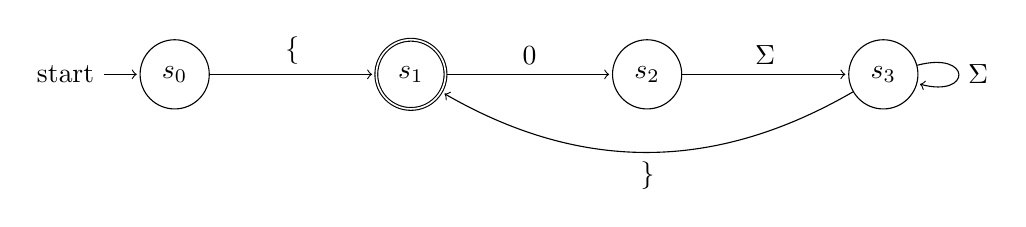
\begin{tikzpicture}[shorten >=1pt,node distance=3cm,on grid,auto] 
        \node[state,initial] (s_0)   {$s_0$}; 
        \node[state,accepting] (s_1) [right=of s_0] {$s_1$};
        \node[state] (s_2) [right=of s_1] {$s_2$}; 
        \node[state,] (s_3) [right=of s_2] {$s_3$}; 
         \path[->] 
         (s_0) edge node {\{ } (s_1)
         (s_1) edge node {0 } (s_2)
         (s_2) edge node {$\Sigma$ } (s_3)
    
         (s_3) edge [bend left, below] node { \} } (s_1)
         (s_3) edge[loop right] node {$\Sigma$ } (s_3);
     \end{tikzpicture}
\end{adjustbox}%

\end{document}